% =========================================================================== %
% TeX input file: "Run the hello world application"
%
% WARNING: this tex file does not compile standalone, it needs to be embedded
% in a master tex document (e.g. Introduction.tex)
% =========================================================================== %

After the initial project creation step we are ready to start the server and the clients of the still empty Scout application.
For this, we switch to the Scout Explorer and select the root node \element{org.eclipse.scout.helloworld}.
Selecting the application's \node{org.eclipse.scout.helloworld} in the Scout Explorer displays the product launchers in the \textit{Scout Object Properties}.
As we can see in \figref{start_client}, we have product launchers for four different development products.

\begin{tabular}{ l l }
  \textbf{Server} & The Scout server application\\
  \textbf{RAP}    & The RAP server application for web and mobile clients\\
  \textbf{Swing}  & The Scout Swing desktop client application\\
  \textbf{SWT}    & The Scout SWT desktop client application\\
\end{tabular}

\begin{figure}
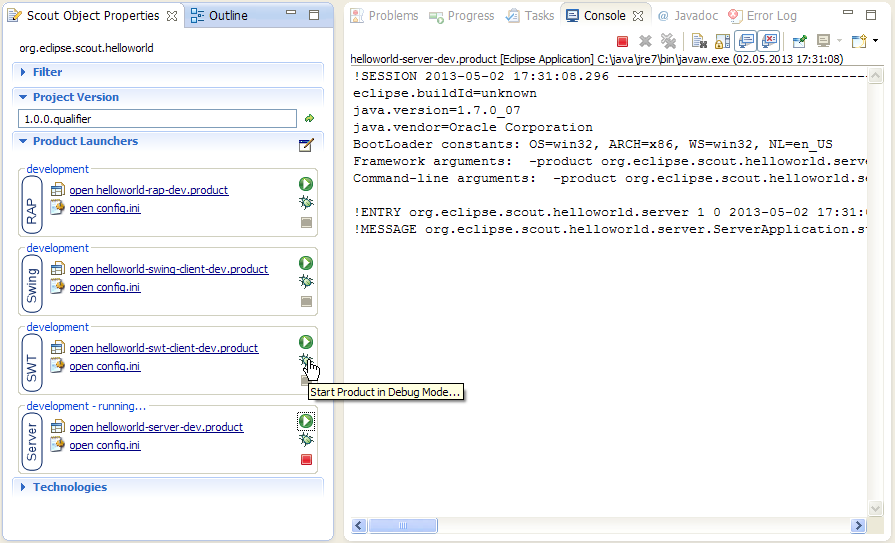
\includegraphics[width=15cm]{sdk_start_client_product.png} 
\caption{Starting the web client in the Scout SDK using the provided RAP product launcher. Make sure to start the server before starting any client product.}
\figlabel{start_client}
\index{Product launchers}
\end{figure}

Each product launcher box provides a link to the corresponding Eclipse product file\footnote{
Product files define the set of all components that are necessary to build the complete application.
},
the configuration file\footnote{
The configuration file \filename{config.ini} provides parameters that are read at startup of the corresponding program.
},
as well as three launcher icons to start and stop the corresponding application.
The green \icon{Circle} starts the product in normal mode.
The \icon{Bug} just below, starts a product in debug mode.
To terminate a running product, the red \icon{Square} is provided. 
Alternatively, you can also stop products by clicking on the same red icon in the console view.
This is shown on the right hand side of \figref{start_client}.
Client products may also be stopped by closing the client's main window or using the provided \menu{File|Exit}.

Before any of the client products is started, we need to start the server product using the green circle or the bug launcher icon.
During startup of the Scout server you should see console output similar to the one shown on the right hand side of \figref{start_client}.
Once the server is running, you may start the web client as shown in \figref{start_client}, the Swing client, or the SWT client in the same way.
And with a running RAP product, the Scout web client can be opened in a web browser.
Just click on the provided \link{Automatic Device Dispatch} or open a a browser and manually type the address \texttt{http://localhost:8082/web} into the browser's navigation bar.

\begin{figure}
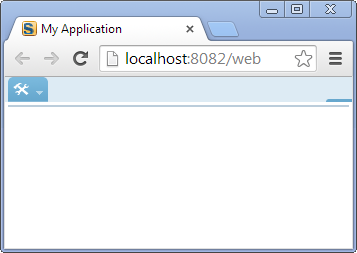
\includegraphics[width=4.5cm]{hellworld_empty_rap.png} \hspace{3mm}
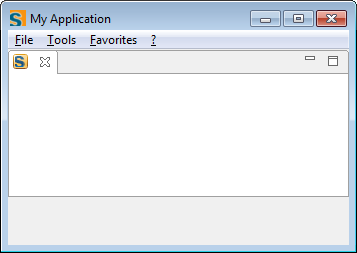
\includegraphics[width=4.5cm]{hellworld_empty_swing.png} \hspace{3mm}
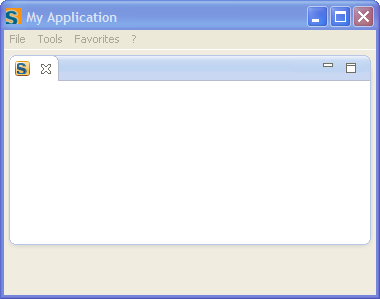
\includegraphics[width=4.5cm]{hellworld_empty_swt.png}
\caption{Running the three client applications. 
Each client displays an empty desktop form. 
From left to right: The web client, the Swing client, and the SWT client}
\figlabel{helloworld_empty}
\end{figure}

Having started the Scout server and all client products, the client applications should become visible as shown in \figref{helloworld_empty}.

% =========================================================================== %
% EOF TeX input file
% =========================================================================== %
